\documentclass[12pt]{article}
    \usepackage{graphicx}
\pagestyle{empty}
\topmargin= -25pt
\textwidth=6 true in
\textheight=9.5 true in
\oddsidemargin = 0.0 true in
\evensidemargin = 0.0 true in
\newcommand{\ul}{\underline}
\newcommand{\spa}{\hspace{.25in}}
\begin{document}

{%\large
\begin{center}
%\mbox{ }
%\vspace{.1in} \\
    Key for Exam I\\
    Computer Science 420 \\
    Dr.~St.~John\\ 
    Lehman College\\
    City University of New York\\ 
    25 March 2003
\end{center}
}

\begin{enumerate}

% 1 T or F
    \item True or False:  {\tt(1 point each)}
    \begin{enumerate}
        \item \underline{\tt\bf T} Every relationship in an E/R diagram must have an attribute.
        \item \underline{\tt\bf F} Subclasses in E/R diagrams are exactly the same as subclasses in Java. 
        \item \underline{\tt\bf T} An entity set can have any number of attributes.
        \item \underline{\tt\bf F}  A relationship connects two or more entity sets.
        \item \underline{\tt\bf F}  To indicate an attribute is a key in an E/R diagram, you circle it.
        \item \underline{\tt\bf F} Attributes that are keys cannot 
		appear in functional dependencies.
        \item \underline{\tt\bf T} A weak entity set depends on another entity set for all or part of its key.
        \item \underline{\tt\bf F} The left side of a multivalued dependency is always a key.
        \item \underline{\tt\bf F} An SQL query can have at most one relation listed in the 
		{\tt FROM} clause.
        \item \underline{\tt\bf F} Views cannot be modified.
    \end{enumerate}

%2 short answer
\item Answer the following in two sentences or less:
\begin{enumerate}
    \item What is the difference between a set and a bag?
	\\
	{\tt  A set has at most one copy of every element, where a bag (or multiset as it's also known),
	can have multiple copies.
	
	(5 points total, partial credit (2 points) for relevant, but not completely correct answer.)
	}
    \item What is the difference between a functional dependency and multivalued dependency?
     	\\
	{\tt A functional dependency says that if two tuples of a relation which agree on some
	particular set of attributes must also agree on some other particular attributes.  A 
	multivalued dependency is a weaker condition that says if two tuples of a relation 
	agree on a particular set of attributes then all possible combinations of this particular
	set (the left hand side of the dependency) and another particular set of attributes
	(the right hand side).
	
	(5 points total, partial credit (2 points) for relevant, but not completely correct answer).}

\end{enumerate}

%3 Java program
\item Write a {\bf complete} Java program ``Help, I'm caught inside a database exam!'' to
the terminal window.

\begin{verbatim}
public class Question3
{  public static void main(String[] args)
   {  System.out.println("Help, I''m caught inside a database exam!");
   }
}\end{verbatim}

{\tt 
(2 points for having a println() but missing the rest of the program,\\
-1 points for missing parentheses or minor syntax errors,\\
-5 points for missing the main() method.)
}
%\newpage
%4 
\item 
  \begin{enumerate}
     \item How many different ways are there to represent a relation instance if that 
        instance has 2 attributes and 2 tuples?
	\\
	{\tt The 2 attributes could be in either order and the tuples could be in either
	order, so, there's $2\times 2 = 4$ possible ways to represent the instance.
	
	(5 points total.  If no explanation, only 1 point partial credit.)
	}
	
     \item How many different ways are there to represent a relation instance if that 
        instance has 3 attributes and 2 tuples?
	\\
	{\tt With 3 attributes, any one of them could be listed first, then of the 
	remaining two, either could be next.  
	So, there's $3\times 2 = 6$ possibilities for the 
	ordering of the attributes.  There's 2 ways to order the tuples.  So, overall,
	there's $2\times 6 = 12$ possible ways to represent the instance.
	
	(5 points total.  If no explanation, only 1 point partial credit.)
	}
	
    \end{enumerate}

%5 FD 
\item For each of the following, indicate whether the statement is {\bf always true}
(for every instance of R), {\bf sometimes true} (that
is, you can find some instance of a relation for which the statement holds), or
{\bf always false} (there is no instance that will make the statement true).\\
Given a relation R(A,B,C):
\begin{enumerate}
    \item If $A \rightarrow B$, then $B \rightarrow A$.
	    
	    Circle one:  ALWAYS TRUE \ \ \ \underline{\bf SOMETIMES TRUE} \ \ \ ALWAYS FALSE
	    
	    {\tt (3 points total, 1 point partial credit for ALWAYS FALSE)}
    \item If $A \rightarrow B$ and $B \rightarrow C$, then $A \rightarrow C$.
	    
	    Circle one:  \underline{\bf ALWAYS TRUE} \ \ \ SOMETIMES TRUE \ \ \ ALWAYS FALSE
	    
	    {\tt (3 points total, 1 point partial credit for SOMETIMES TRUE)}
    \item If $A \rightarrow B$ is the only functional dependency, then BC is a key. 
	    
	    Circle one:  ALWAYS TRUE \ \ \ SOMETIMES TRUE \ \ \ \underline{\bf ALWAYS FALSE}
	    
	    {\tt (3 points total, 1 point partial credit for SOMETIMES TRUE)}
\end{enumerate}

%6 1-1, m-1, m-m question
\item For each of the following types of situations, give an
	example {\bf and} draws its E/R diagram:
	
	{\tt (5 points each.  No points taken off for missing arrows or keys.\\
	-2 points for wrong example,\\
	-2 points for missing relationship (diamond).)
	}
	
    \begin{enumerate}
	\item a many-one relationship:
	
		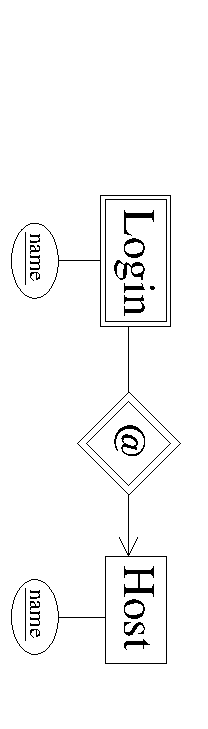
\includegraphics[height=2in, angle=90]{login_weakES.pdf}
	
	\item an one-one relationship:
	
	\hspace{.5in}	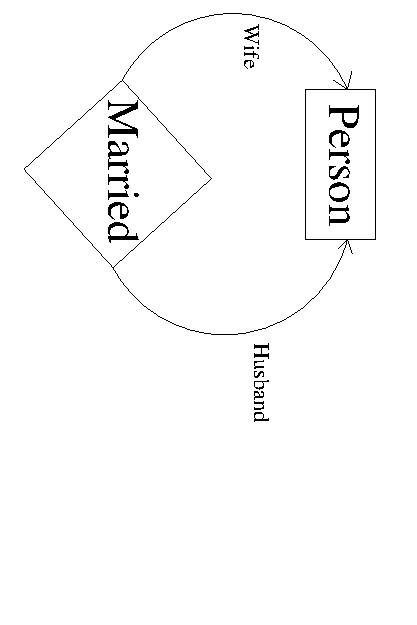
\includegraphics[height=1.5in, angle=90]{married.pdf}
	
    \end{enumerate}

%\newpage

%7 From an E/R diagram, give keys specified and translate into
% database schema
\item
\begin{enumerate}
    \item Draw an E/R diagram for the following situations. Indicate any
	keys, weak entity sets, or subclasses:\\
        Entity sets {\em Movies}, {\em Stars} and {\em Studios}.  
    	A movie has a title, year (in which the movie was made), the length, and
         the film type (either ``color'' or ``blackAndWhite'').  The other two entity
	sets both have the same attributes: their name and their address.
	Stars can star in movies.  Movies are owned by studios. 
	
	{\tt (5 points.  See p 26 for diagram.)}
	
    \item Translate your E/R diagram into a relation schema.  Indicate
	keys for each relation as well as any functional dependencies that
	hold about each relation.
	
	{\tt (7 points.  See Example 3.1 on p 67 for relation schema and 
	Examples 3.16 and 3.17 on p 87-88 for functional dependencies.)}
	
    \item Write the SQL statement that will create the Stars table above.
    
	{\tt (4 points)}
\begin{verbatim}	
  CREATE TABLE Stars(
    name char(30),
    address varchar(50),	
  };
\end{verbatim}

    \item Write the SQL statements that add the following stars to your table that
	keeps track of stars:
\begin{verbatim}
Harrison Ford, 123 Maple Street
Carrie Fisher, 456 Broadway
\end{verbatim}
    
	{\tt (4 points)}
\begin{verbatim}	
  INSERT INTO Stars(name, address) 
         VALUES('Harrison Ford', '123 Maple Street');
  INSERT INTO Stars(name, address) 
         VALUES('Carrie Fisher', '456 Broadway');
\end{verbatim}
\end{enumerate}

%\newpage
%8 BCNF and 4NF
\item Given the relation schema $R(A,B,C,D)$ with the functional dependencies
$$
\begin{array}{c}
	AB \rightarrow C\\
	C \rightarrow D\\
	D \rightarrow A\\
\end{array}
$$
\begin{enumerate}
    \item What are the keys of $R$?  
    	{\tt
	Note that any key must include B, since there's no way to derive B from the functional 
	dependencies that yield B.  So, we only need to check the closure of subsets that
	contain B:
	$$
	\begin{array}{lll}
	A^+ = A 		& AB^+ = ABCD & ABC^+ = ABCD\\
	B^+ = B 		& BC^+ = ABCD & ABD^+ = ABCD\\
	C^+ = ACD 	& BD^+ = ABCD & BCD^+ = ABCD\\
	D^+ = D 		 \\	
	\end{array}
	$$
	This gives superkeys of AB, BC, BD, ABC, ABD, BCD, and ABCD, and
	keys of AB, BC, and BD.
	
	(4 points total. \\
	-1 point for each missing key.)
	}
    \item Indicate all the Boyce Codd Normal Form violations.  
	Do not forget to consider
	dependencies that are not in the given set, but follow from them.
	However, it is not necessary to give violations that have more than
	one attribute on the right side.
	
	{\tt
	C $\rightarrow$ D, 
	D $\rightarrow$ A, 
	C $\rightarrow$ A, 

	(3 points total.)
	}
	
    \item Decompose the relations, as necessary, into a collection of 
	relations that are in {\bf Boyce Codd Normal Form}.
	{\tt
	
	Decomposing around the BCNF violation, C $\rightarrow$ D,
	gives the smaller relations wtih functional dependencies:
	$$
	\begin{array}{ll}
	R_1(C,D) & R_2(C,A,B)\\
	C \rightarrow D & AB \rightarrow C\\
				& C   \rightarrow A\\
	\end{array}
	$$
	The key for $R_1$ is C, so $R_1$ is in BCNF.\\
	The key for $R_2$ is AB, so C $\rightarrow$ A is a BCNF violation.
	Decomposing $R_2$ gives:
	$$
	\begin{array}{ll}
	R_3(C,A) & R_4(C,B)\\
	C \rightarrow A & \\
	\end{array}
	$$
	
	(3 points total.)
	}
\end{enumerate}

%9 sql
%\newpage
\item Given the company database used in laboratory exercises with
the relations:
\begin{verbatim}companies (co_id serial,
   co_name varchar(64),
   co_postcode varchar(16),
   co_lastchg timestamp );
products (pr_code varchar(6) PRIMARY KEY,
   pr_desc varchar(64));
orders (ord_id serial,
   ord_company int4 REFERENCES companies(co_id),
   ord_product varchar(6) REFERENCES products(pr_code),
   ord_qty int4,
   ord_placed date,
   ord_delivered date,
   ord_paid date);\end{verbatim}
Write SQL queries that:
\begin{enumerate}
   \item gives the product codes contained in the database:
 
 \begin{verbatim}
 SELECT pr_code FROM products;\end{verbatim}  	
	{\tt
	(2 points)
	}
	
   \item gives the product codes and the minimum number order, 
	the average number ordered, and the maximum number ordered:
	
 \begin{verbatim}
 SELECT ord_product, MIN(ord_qty), AVG(ord_qty), MAX(ord_qty) 
 FROM orders
 GROUP BY ord_product; \end{verbatim}  		
	{\tt
	(3 points)
	}
	
   \item list all orders that not been paid for:
	
 \begin{verbatim}
 SELECT * 
 FROM orders
 WHERE ord_paid = NULL; \end{verbatim}  	
	
	{\tt
	(2 points)
	}
	
   \item find each order and its quantity that exceeds the average order 
	quantity for all orders:
	
 \begin{verbatim}
 SELECT * 
 FROM orders
 WHERE ord_qty > SELECT AVG(ord_qty) FROM orders;\end{verbatim}  	
	{\tt
	(3 points)
	}
	
\end{enumerate}
                           



\end{enumerate}
\end{document}


